\documentclass{beamer}

\usetheme{Warsaw}
%\usepackage[spanish]{babel}
\usepackage[latin1]{inputenc}
%\usepackage{algorithm}
%\usepackage{algorithmic}
\usepackage{verbatim}
\usepackage{amsbsy}
\usepackage{amsfonts}
\usepackage{amssymb}
\usepackage{multirow}
%\usepackage[dvipdf]{graphicx}

\setbeamercovered{transparent}

\newcommand{\?}{?`}
\newtheorem{definicion}{Definici\'on}

\mode<presentation>
{
  \setbeamertemplate{background canvas}[vertical shading][bottom=white!10,top=blue!10]
  \setbeamercolor{itemize item}{fg=red}
  \usetheme{CambridgeUS}
  \usefonttheme[onlysmall]{structurebold}
}

%
% The following info should normally be given in you main file:
%

\title[VAR-PLS]{VAR-PLS}
\author[GGF, FCV, JG] {Graciela Gonz\'alez Far\' ias}
\institute[CIMAT MTY]{CIMAT Monterrey\\
Monterrey, NL.}
\date{June 2012}


\begin{document}


%\frame{\titlepage}

%%%%%%%%%%%%%%%%%%%%%%%%%%%%%%%%%%%%%%%%%%

\begin{frame}
  \begin{center}
    % \vspace{8mm}
    \begin{block}{}
      \begin{center}
        \vspace{3mm}
        {\Large Var PLS}
        \vspace{3mm}
      \end{center}
    \end{block}
    \vspace{5mm}
    Graciela Gonz\'alez Far\'ias \\
    \vspace{5mm}
    {\small Francisco Corona and Jes\'us Gonzalo \\
    Centro de Investigaci\'on en Matem\'aticas,
      Campus Monterrey\\
      ISBIS 2012\\
      Bangkok, Thailand, June 17, 2012}
    \vspace{5mm}
  \end{center}
\end{frame}


\begin{frame}{Contenido}
  \begin{itemize}
  \item Motivation
  \item PLSAR and PLS
  \item Quick overview of VAR Models
  \item Definition for VAR-PLS
  \item Bootstrap for VAR-PLS
  \item Conclusions
  \end{itemize}
\end{frame}


\begin{frame}{Motivaci\'on}
  \begin{itemize}
    \item PLS is a technique that has bee proven its impact on many applications such as quality control starting with the Chemistry, batch processes, medical images analysis, microarrays, path modeling, classification, discrimination, spacio-temporal PLS models just to mention some, with authors such as McGregor, Nomikos, MacIntosh, V. Esposito Vinz, P. Garthwaite, and so on 
    \item The method can be used in univariate and multivariate data as well
    \item {\it{It has been shown that gives better prediction even when the standard assumptions are met}}
    \item Phillip Hans Franses (2006) propose a methodology to construct the forecast $h$ steps ahead in an optimal way, through an autoregresive order $p$:  {\it{An Autoregresive Partial Least Square denote as  $PLSAR(h,p)$}}
      \end{itemize}
    \end{frame}

\begin{frame}{Our case of interest}
  \begin{itemize}
    \item Develop a model to predict the Mexican inflation, as precise as possible
    \item The model has to consider, as the principal source of the mexican inflation, the grow and the variation on the monetary condition of the country
    \item Irrespective of all possible discussions, there seems to be a common understanding to belived that the inflationary process, in the lung run, is a purely monetary fenomena
    \item Here we are not taking the discussion on the existence or not of such relationship but we will show its empirical properties with a model that is tested out of the sample via its error prediction measure
    
  \end{itemize}
\end{frame}

\begin{frame}{Our case of interest}
  We work with 4 indexes ( we bulit those) from January 2000 to Feb 2012
  \bigskip
  
  \begin{itemize}
    \item $p$: Consumer price index  
    \bigskip
    \item $m0$: Monetary base 
      \bigskip
    \item $r$: Equilibrium interest rate (28 days)
      \bigskip
    \item $y$: Industrial production index 
  \end{itemize}
\end{frame}

\begin{frame}{Nuestro caso de inter\'es}
  \begin{figure}[htbp]
    \center{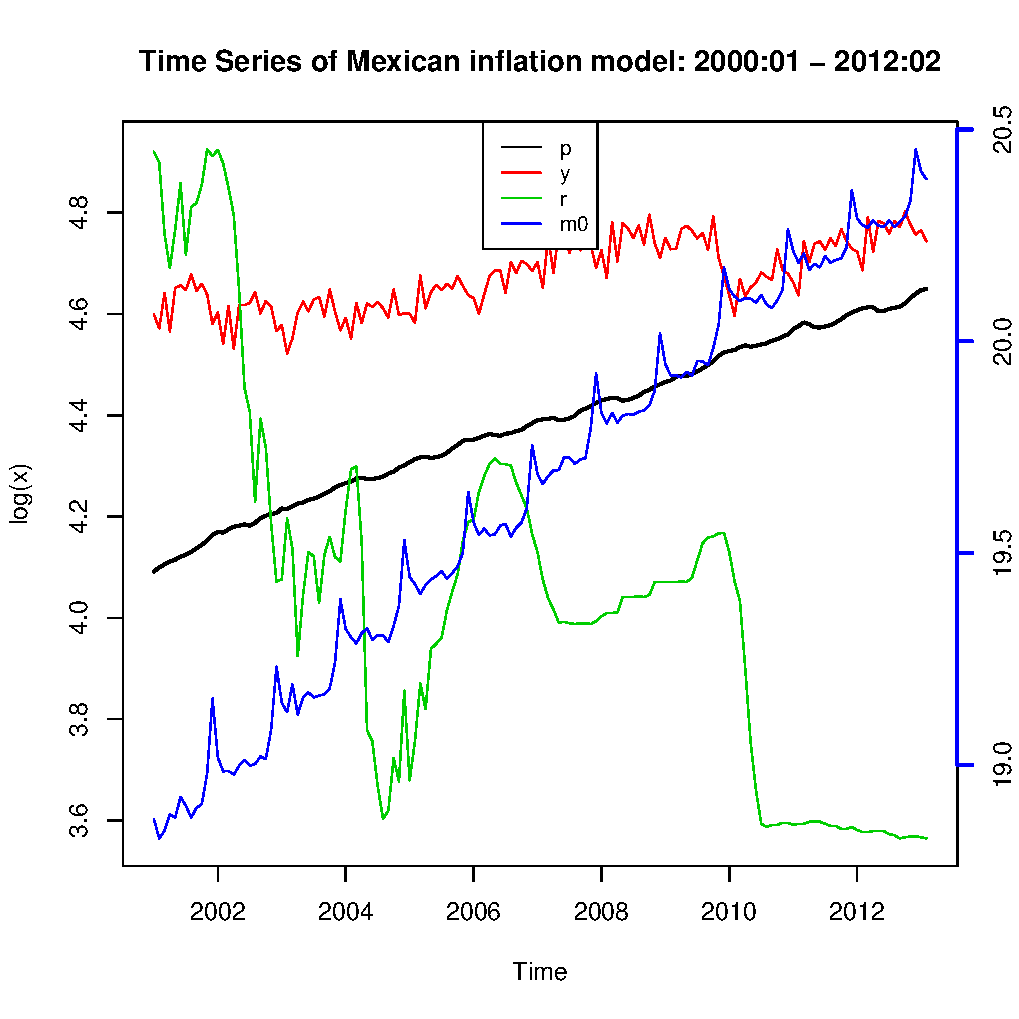
\includegraphics[scale=0.5]
      {figs/graph_1_v2.pdf}}
\end{figure}
\end{frame}

\begin{frame}{Our case of interest}
  \begin{itemize}
    \item We generalized the work proposed by Franses in the following way:
    \bigskip
    
      \begin{enumerate}
      \item Give a multivariate representation based on the flexibility of the $VAR$ models, model that we will call $VAR-PLS(h,p)$
      \item Extend the model to consider deterministic variables (dummies, trend, etc.) as well as exogenous variables
      \item Bootstrap prediction intervals
      \item Compare the forecast capabilities between a $VAR-PLS(h,p)$ and a forecast $VAR$ model explicitly built for (integral predictor method)
            \end{enumerate}
  \end{itemize}
\end{frame}

\begin{frame}{}
  \begin{block}{}
    \begin{center}
      \vspace{3mm}
      {\Large $PLSAR(h,p)$}
      \vspace{3mm}
    \end{center}
  \end{block}
\end{frame}

\begin{frame}{$PLSAR(h,p)$}
  Franses three different ways to construct a forecast for an $AR(p)$:
  \bigskip
  \begin{itemize}
    \item[\textbf{1-}] A single model for all horizons , an iterative procedure will come on hand
      \begin{displaymath}
        AR(p): y_{T+h}=\mu+
        \rho_1y_{T+h-1}+\rho_2y_{T+h-2}+\cdots + \rho_py_{T+h-p} + \epsilon_T
      \end{displaymath}
      
      For the $AR(p)$ the classical procedure to get $h$
      step ahead forecast, plus the fact that we estimate the parameters (OLS).
  \end{itemize}
\end{frame}

\begin{frame}{$PLSAR(h,p)$}
  \begin{itemize}
  \item[\textbf{2-}] One model for each horizon, the variance will vary within each horizon and {\it{one can count with different models for each step}}
  \bigskip
    \begin{displaymath}
      AR_h(p): y_{t+h}=\mu+
      \rho_{1,h}y_{t}+\rho_{2,h}y_{t-1}+\cdots + \rho_py_{t-p}+\epsilon_{t,h}
    \end{displaymath}
    The $AR_h(p)$  is an alternative to the $AR(p)$ because
    \begin{itemize}
    \item OLS minimize the sum of square of $\epsilon_t$  but there is no way to assure it will remain minimum for all the $h$ steps in the future 
    \item For stationary time series recall the the forecast of an  $AR(p)$ model quickly converge to the inconditional mean (and variance, for the interval prediction error) clearly depending on  
    $h\geq p$
        \item For more details on this type of models see : Pesaran \& Pick (2010), Marcellino, Stock \& Watson (2004), Carreiro, Kapetorios \& Marcellino (2010), Tiao \& Xu (1993) among others.
    \end{itemize}
  \end{itemize}
\end{frame}

\begin{frame}{$PLSAR(h,p)$}
  \begin{itemize}
  \item[\textbf{3-}] Something in between: $PLSAR$, this model behaves like {\it{ in the middle }}between an $AR(p)$ and a $AR_h(p)$  
    \begin{displaymath}
      PLSAR(h,p): \hat{Y}=XB_{PLS}
    \end{displaymath}
    \begin{itemize}
    \item It is clear that exists adjacent correlation between the time series, and neither one of the above models take them into account. In other words, we know that $(y_t,y_{t-j})$ are correlated and so are $(y_{T+h},y_{T+h-j})$, . Therefore we would like to jointly predict $(y_{t+h},y_{t+h-1},y_{t+h-2},\ldots,y_{t+1})$ through $(y_{t},y_{t-1},y_{t-2},\ldots,y_{t-p})$. PLS is a techinique very atractive to do so.
    \end{itemize}
  \end{itemize}
\end{frame}

\begin{frame}{$PLSAR(h,p)$}
  \begin{itemize}
  \item[\textbf{3-}]   Franses propose to arrange the information as 

      \begin{displaymath}
        (y_{t},y_{t-1},y_{t-2},\ldots,y_{t-p}) \text{ as the predictor matrix
           } X
      \end{displaymath}
      \begin{displaymath}
        (y_{t+h},y_{t+h-1},y_{t+h-2},\ldots,y_{t+1})
        \text{ as the predicted matrix } Y
      \end{displaymath}
      \bigskip
      \item Applied the $PLS$ algorithm, to get the latent variables with the relevant information given in $X $ and $Y$.
      \medskip
     \item His simulations shows that the $PLSAR(h,p)$ is quite competitive with respect to the classical models in the literature
  \end{itemize}
\end{frame}

\begin{frame}{}
  \begin{block}{}
    \begin{center}
      \vspace{3mm}
      {\Large $PLS$}
      \vspace{3mm}
    \end{center}
  \end{block}
\end{frame}

\begin{frame}{PLS}
  \begin{itemize}
  \item PLS can be tract from different stand points, to us the relationship between its linear expression  will be the best one, in order to related with a Vector Autoregresive model   
   \bigskip
  
   \begin{displaymath}
      Y=XB+U,
    \end{displaymath}
    \bigskip
    where $Y$ is a $N\times k$ matrix, $X$ is $N\times p$, $B$ is a
     $p\times k$ matrix, and  $U$ is  $N\times k$.


  \end{itemize}
\end{frame}


 
\begin{frame}{PLS}
  \begin{itemize}
  \item The basic procedure maximize the  
    \begin{displaymath}
      \max cov(X\alpha,Y\beta)^2
    \end{displaymath}
    under certain restrictions,
    \begin{displaymath}
      \alpha'(S_{xx}^{*}+\lambda_x)\alpha = 1 \quad \text{and } \quad
      \beta'(S_{yy}^{*}+\lambda_y)\beta = 1 
    \end{displaymath}
    donde $S_{xx}^{*}=(1-\lambda_x)S_{xx}$ and
    $S_{yy}^{*}=(1-\lambda_y)S_{yy}$.
    \begin{itemize}
    \item $(X\alpha,Y\beta)$ are linear combinations of the variables that  maximize the covariance or actually the squere covariance (the sign is not important just the direction)
    \item $S_{xx}$ and $S_{yy}$ the varince covariance matrices
      , $\beta'\beta=1$ y $a'S_{xx}a=1$.
    \end{itemize}
  \end{itemize}
\end{frame}
 
\begin{frame}{PLS}
  \begin{itemize}
  \item We maximze the the objective function:
    \begin{displaymath}
      \mathcal{L}=
      (\alpha'S_{xy}\beta)^2-\gamma(\alpha'(S_{xx}+\lambda_x)\alpha-1)
      - \mu(\beta'(S_{yy}+\lambda_y)\beta-1).
    \end{displaymath}
  \item After some algebra we get the {\textcolor{blue}{scores}} for  $X$ y
    $Y$, $t=Xw=Ew$ and $u=Yq=Fq$.
  \item  Normalizing the scores   $t=t/\sqrt{t't}$, and after simplifications and more algebra we get the \textcolor{red}{loadings} for  $X$ and $Y$: $p=E't$
   and $q=F't$.
  \end{itemize}
\end{frame}
 
\begin{frame}{PLS}
  \begin{itemize}
  \item Writing in matrix form $w,t,p$ y $q$ we get $R=W(P'W)^{-1}$ and
   finally
    \begin{displaymath}
      Y=XB+U, \text{ then} \hat{Y}=XB_{PLS},
    \end{displaymath}
    where $B_{PLS}=R\textcolor{blue}{(T'T)^{-1}T'Y}=RQ'$.
  \item     \bigskip

    For a nice introduction see P.H. Garthwaite
    (1994). An Interpretation of Partial Least Squares. JASA Vol 89,
    No 425, pp 122-127 and A. Hoskuldsson (1988). PLS Regression Methods. Journal of
    Chemometrics, Vol 2, pp 221-228.\\
    \medskip
    \textcolor{blue}{Note}: Franses shows that if  the $B_{PLS}$ matrix has full rank it implies a different model for
each of the columns of $Y$ , and hence a model like $AR_{h,p}$. In the exceptional case that
$B_{PLS}$ has rank 1, then the $AR(p)$ appears.
  \end{itemize}
\end{frame}

\begin{frame}{}
  \begin{block}{}
    \begin{center}
      \vspace{3mm}
      {\Large Vector Autoregressive models and PLS}
      \vspace{3mm}
    \end{center}
  \end{block}
\end{frame}

\begin{frame}{$VAR-PLS$}
  A $VAR(p)$ processes is defined as
    \begin{displaymath}
      y_t=A_1y_{t-1} + A_2y_{t-2} + \cdots + A_py_{t-p} + CD_t + u_t,
    \end{displaymath}
  where
    \begin{itemize}
    \item $A_i$, $i=1,2,\ldots, p$, the coefficient matrix
    \item $u_t$ a white noise process
     with variance covariance given by $\Sigma_u=E(u_t,u_t')$
    \item $C$  matrix of regressor coefficients for deterministc factors
            \item $D_t$ the vector of deterministic factors
    \end{itemize}
\end{frame}

\begin{frame}{$VAR-PLS$}
  We also know that a $Var(p)$ can be written as a $Var(1)$ as follows
    \begin{displaymath}
      Y_t=AY_{t-1} + V_t,
    \end{displaymath}
    con
    \begin{small}
    \begin{displaymath}
      Y_t=\left(
        \begin{array}{c}
          y_t \\
          y_{t-1} \\
          \vdots \\
          y_{t-p+1}
        \end{array}
        \right), \quad
        A=\left(
        \begin{array}{ccccc}
          A_1 & A_2 & \cdots & A_{p-1} & A_p \\
          I & 0 & \cdots & 0 & 0 \\
          0 & I & \cdots & 0 & 0 \\
          \vdots & \vdots & \ddots & \vdots & \vdots \\
          0 & 0 & \cdots & I & 0
        \end{array}
        \right), \quad
        V_t=\left(
        \begin{array}{c}
          u_t \\
          0 \\
          \vdots \\
          0
        \end{array}
        \right).
    \end{displaymath}
    \end{small}
   If the eigenvalues of  $A$ are less than one, then the $VAR(p)$ is stable
\end{frame}

\begin{frame}{$VAR-PLS$}
  \begin{itemize}
  \item We use the VAR representation to determine the order of the model 
  
  \item The general procedure is quite standard. Order  $p=0,\ldots,p_{\max}$ and choose the value of $p$ that minimize some criteria. The criteria are usually written as:
     \begin{displaymath}
      IC(p)-\log \vert \hat{\Sigma(p)} \vert + C_T \varphi(K,p),
    \end{displaymath}
    where
    \begin{itemize}
      \item $\hat{\Sigma(p)}=T^{-1} \sum_{i=1}^T\hat{u}_t'\hat{u}_t$,
      \item $C_T$ an indexed sequence of the size  $T$
      \item $\varphi(K,p)$ is a penalty function that involves the order of the $VAR(p)$
    \end{itemize}
  \end{itemize}
\end{frame}

\begin{frame}{$VAR-PLS$}
  \begin{itemize}
  \item The most common information criterias are: Akaike (AIC), Schwarz-Bayesiano (BIC), Hannan-Quinn (HQ) and Final predicction error (FPE):
    \begin{itemize}
    \item Akaike: $AIC(p)=\vert \hat{\Sigma(p)} \vert +
      \frac{2}{t}pK^2$
    \item Schwartz-Bayesiano: $BIC(p)=\vert \hat{\Sigma(p)} \vert +
      \frac{\log T}{t}pK^2$
    \item Hannan-Quinn: $HQ(p)=\vert \hat{\Sigma(p)} \vert +
      \frac{2\log T}{t}pK^2$
    \item Final prediction error:
      $FPE(p)=\left(\frac{T+p^{*}}{T-p^{*}}\right)^K
      \text{det}(\hat{\Sigma(p)})$  
    \end{itemize}
  \item The AIC asymptotically overestimate the order of the model with a positive 
  probability whereas BIC and HQ are consisten estimator of the order if,  the real value of is less than or equal than $p_max$  \end{itemize}
\end{frame}

\begin{frame}{$VAR-PLS$}
  As for the univariate case, we can built the forecast with a \textcolor{blue}{recursive method:} 
    \begin{displaymath}
    y_{T+h\setminus T}=A_1y_{T+h-1} + \cdots + A_py_{T+h-p} + CD_{T+h}
  \end{displaymath}
  \begin{itemize}
  \item We estimate $A_i$ throught OLS
    \begin{displaymath}
        vec(\hat{A})=\left(
        \begin{array}{c}
          \hat{A}_1 \\
          \vdots \\
          \hat{A}_p
        \end{array}
        \right).      
    \end{displaymath}
  \end{itemize}
\end{frame}

\begin{frame}{$VAR-PLS$}
  \begin{itemize}
  \item 	Under stationarty and ergodicity conditions  for the VAR model (see Hamilton (1994), Lutkepohl (1991) among others), $vec(\hat{A})$ is consistent and asymtotically distributued with covariance matrix given by 
    \begin{displaymath}
      \widehat{var}\left(vec(\hat{A})\right)=\hat{\Sigma} \otimes
      (Z'Z)^{-1},
    \end{displaymath}
    where
    \begin{displaymath}
      \hat{\Sigma}=\frac{\sum_{t=1}^T\hat{\epsilon}_t'\hat{\epsilon}_t}{T-K}
    \end{displaymath}
    and
    \begin{displaymath}
      \hat{\epsilon}_t=Y_t-\hat{A}'Z_t=Y_t-\hat{A}'Y_t
    \end{displaymath}
    the OLS residual at time $t$.
  \end{itemize}
\end{frame}

\begin{frame}{$VAR-PLS$}
  \begin{itemize}
  \item El $i-th$ element of $vec(\hat{A})$ is asymptotically normal (for an a stable $VAR$) and the standard error are the square roots of the diagonal elements of  $\hat{\Sigma}
    \otimes (Z'Z)^{-1}$.
    \item  The $t-test$ for the estimated coefficients are asymptotically correct
    \item Other important situation for the $VAR$ models is the presence of one or more unit roots for the $y_j'$.  From the point of view of the economic theory it mean the study of a \textcolor{blue}{lung run behavior plus the temporal dynamic of the series}. 
      \end{itemize}
\end{frame}

\begin{frame}{$VAR-PLS$}
    \begin{itemize}
  \item \textbf{Cointegration: } The components of a $k-$dimensional vector  $y_t$ are cointegrated of order  $(d,b)$,   denoted by  $y_t\sim CI(d,b)$,  if
  \bigskip 
    \begin{enumerate}
    \item all  components of $y_t\sim$ are $I(d)$
    \bigskip
    \item there exist a vector $\beta\neq 0$ such that  $z_t=\beta'y_t\sim
      I(d-b)$, $b>0$. The vector $\beta$ is called the cointegration vector
      (Lutkepohl, 1991)
          \end{enumerate}
  \end{itemize}
\end{frame}

\begin{frame}{$VAR-PLS$}
  The $VAR(p)$ model can be written as  \textcolor{blue}{Transitory - Vector Error Correction Model ($VECM$)} 
  \begin{displaymath}
    \Delta y_{t}=\Pi  \textcolor{blue}{ y_{t-1}}+\Gamma_1 \Delta y_{t-1} + \cdots +
    \Gamma_{p-1} \Delta y_{t-p+1} + CD_t + u_t,
  \end{displaymath}
  where $\Gamma_i=-(A_{i+1}+\cdots + A_p)$, for $i=1,\ldots ,p-1$ and
  $\Pi=-(I-A_1-A_2-\cdots - A_p)$. 
  
\bigskip

  Or as a  \textcolor{red}{Lung run - Vector Error Correction Model ($VECM$)} 
  \begin{displaymath}
    \Delta y_t=\Pi \textcolor{red}{ y_{t-p}}+\Gamma_1 \Delta y_{t-1} + \cdots +
    \Gamma_{p-1} \Delta y_{t-p+1} + CD_t + u_t,
  \end{displaymath}
  donde $\Gamma_i=-(I-A_{1}-A_2-\cdots -A_i)$, para $i=1,\ldots ,p-1$
  y $\Pi=-(I-A_1-A_2-\cdots - A_p)$. 
\end{frame}

\begin{frame}{$VAR-PLS$}
  The matrix $\Pi$ has the following characteristics:
  \begin{enumerate}
  \item  \textcolor{blue}{$rk(\Pi)=n$},  the $n$ linear combinations are stationary; 
  in other words the $VECM$ is no more than a $VAR$ model in levels
  \item  \textcolor{blue}{$rk(\Pi)=0$}, there is no linear combination that makes $\Pi y_{(t-1)}$ stationary, except for the trivial solution  {\it{i.e.}}, it becomes and $VAR(p-1)$ in first differences  
    \item  \textcolor{blue}{$0<rk(\Pi)<n$}, in this case $\Pi=\alpha \beta'$ ($\alpha$ and $\beta$ with
    dimensions $n\times r$) and $\beta' y_{t-1}$ is stationary. Each
   column of $\beta$ represent a lung run relationship
  \end{enumerate}
\medskip
 \textcolor{blue}{ \it{If the objective is to forecast series that are integrated or cointegrated working with a $VAR$ representation is quite appropriated (see Lutkepohl 2006) }}
\end{frame}

\begin{frame}{$VAR$ Example}
  
  \begin{itemize}
  \item For the mexican inflation example we specify the order of the model through the final error prediction criteria, it was \textcolor{blue}{$p=2$}
  \item We also performed  Johansen test to determine the presence of lung run relationship. Finding the following relationship which it was significant to  $1\%$, level
      \begin{displaymath}
      price+9.68-0.43m-0.89y+0.1r=0
    \end{displaymath}
  \item This relationship is congruent with the economic theory behind it. The inflationary movement increases for the monetary grow, the exceed on demand and the reduction on the money cost 

  \end{itemize}
\end{frame}

\begin{frame}{}
  \begin{block}{}
    \begin{center}
      \vspace{3mm}
      {\Large $VAR-PLS(h,p)$}
      \vspace{3mm}
    \end{center}
  \end{block}
\end{frame}


\begin{frame}{$VAR-PLS(h,p)$}
  \begin{itemize}
  \item The $VAR$ model will give us the DGP
  \bigskip
  \item The $VAR$ model will provide the autoregressive process that we will use to built the $PLS$ regression 
  \bigskip
  \item We built then the matrices in at natural way as:
  \end{itemize}
\end{frame}

\begin{frame}{$VAR-PLS(h,p)$}
  \begin{itemize}
  \item For the $X$ matrix we include the lag vector
      \begin{displaymath}
      X=Y_{t-1}=\left(
        \begin{array}{c}
          y_{t-1} \\
          y_{t-2} \\
          \vdots \\
          y_{t-p}
        \end{array}
      \right), 
    \end{displaymath}
  \item For the $Y$ the observation until time $t$ :
    \begin{displaymath}
      Y=Y_{t}=\left(
        \begin{array}{c}
          y_t \\
          y_{t-1} \\
          \vdots \\
          y_{t-p+1}
        \end{array}
      \right), 
    \end{displaymath}
    using the $X$ matrix with all the lags consider for the DGP.
  \end{itemize}
\end{frame}

\begin{frame}{$VAR-PLS(h,p)$}
  \begin{itemize}
  \item We can introduce exogenous variables with a $C$ matrix, then
      \begin{footnotesize}
    \begin{displaymath}
      X=Y_{t-1}^{*}=\left(
        \begin{array}{c}
          y_{t-1} \\
          y_{t-2} \\
          \vdots \\
          y_{t-p} \\
          D_t
        \end{array}
      \right), 
    \end{displaymath}
    and then, the matrix of coefficients
    \begin{displaymath}
      A^{*}=\left(
        \begin{array}{cccccc}
          A_1 & A_2 & \cdots & A_{p-1} & A_p & C \\
          I & 0 & \cdots & 0 & 0 & 0 \\
          0 & I & \cdots & 0 & 0 & 0 \\
          \vdots & \vdots & \ddots & \vdots & \vdots \\
          0 & 0 & \cdots & I & 0 & 0
        \end{array}
        \right)
    \end{displaymath}
    \end{footnotesize}
  \item Those are the basic ingredients for a  $VAR-PLSX$ that will allows to predict $h$ steps ahead 
  \end{itemize}
\end{frame}

\begin{frame}{$VAR-PLS(h,p)$ Example}
 For the $VAR(p=3)-PLS(h=24,j)$
  \begin{itemize}
  \item We kept 24 observation to have a long horizon of possible comparisons 
  \item We consider dummies for the monthly effects
  \item For the optimal $p$ we estimate $VAR-PLS$,  we use R to fit 
  
  $$Y_{t,119\times 4} = X_{t,119\times 23} B_{23\times 4}+ U_{t,119\times 4}$$ 
  
and estimate it and predict for the $VAR(3)-PLS(24,j)$ in a recursive way as in the $VAR(p)$. (The last component agrees with the VAR(p) OLS estimate) 
  \item For the $pK+g=23$ components and the 24 out of the 
  sample observations we get the MAPE to make the comparison
  \end{itemize}
\end{frame}

\begin{frame}{$VAR(p)$ forecast}
  Para el modelo $VAR(p=3)$
  \begin{itemize}
  \item Combining all the variables estimate our  
    $VAR_j(p)$, $j=1,2,\ldots,3696$
  \item For the 24 steps out of the sample we use 7 different criteria to measure the behavior of the forecast (Hyndman \& Koehler 2006):    
  \begin{itemize}
    \item MAPE: Mean Absolute Percentage Error
    \item MdAPE: Median Absolute Percentage Error
    \item RMSPE: Root Mean Square Percentage Error
    \item RMdSPE: Root Median Square Percentage Error
    \item MRAE: Mean Relative Absolute Error
    \item MdRAE: Median Relative Absolute Error
    \item GMRAE: Geometric Mean Absolute Error
    \end{itemize}
  \end{itemize}
\end{frame}

\begin{frame}{$VAR-PLS(h,p)$}
  \begin{itemize}
  \item For the last 3 we need to work with a benchmark model (autoregressive order 1) and for            $i=1,\ldots,24$ $(h = 24)$ obtain the statistic:
      \begin{displaymath}
      test=\frac{Y_{t-i}-Y_{t+i,VAR_j(p)}^f}{Y_{t+i}-Y_{t+i,AR(1)}^f}
    \end{displaymath}
  \item \textcolor{blue}{With the 7 criteria, integrate the forecast to one by taking  the 0.5 quantile} for the horizon consider, repeat it for their upper and lower confidence intervals to get the predicted integral interval
  \end{itemize}
\end{frame}

\begin{frame}{}
  \begin{block}{}
    \begin{center}
      \vspace{3mm}
      {\Large Prediction Interval: VAR-PLS}
      \vspace{3mm}
    \end{center}
  \end{block}
\end{frame}

\begin{frame}{$VAR-PLS(h,p)$ : Bootstrap}
\bigskip
  We also have to construct the prediction intervals for the VAR-PLS model.\\
  
\bigskip
  
We use a similar procedure to the one proposed by Pascual, Ru\'iz and Fresoli (2011). Bootstrap forecast of multivariate VAR models without using the backward representation. Working Paper 11-34, Statistics and Econometrics Series. \\

They use the seminal ideas of Kim (2001and some results from a previous work,  Pascual, L., J. Romo, and E. Ruiz (2004a). Bootstrap predictive inference for ARIMA processes, Journal of Time Series Analysis, 25, 449-465)
\end{frame}

\begin{frame}{$VAR-PLS(h,p)$ : Bootstrap}
For the  VAR model they proposed a method that coupes with:
 \medskip
   \begin{enumerate}
  \item The uncertainty give by the estimation of the parameter, building confidence regions using their bootstrap method    
  \begin{itemize}
    \item {\it{This regions are valid under Gaussian assumptions (L\"utkepolh et al, 1991), even though do not reflect, for small sample size, the asymmetric distribution of the predicted values (under estimated parameters)}}
    \end{itemize}
  \item The backward representation makes calculations quite complicate more in the case of the $VAR(p)$ representation and $p$ taking values greater than 5 for example, which is very common. 
    \begin{itemize}
    \item {\it{``Pascual et al shows that the backward representation can be avoided without loosing the good properties of the bootstrap procedure''   }}
    \end{itemize}
  \end{enumerate}
\end{frame}

\begin{frame}{$VAR-PLS(h,p)$ : Bootstrap}
  Of course we needed to adequate the procedure to the procedure to the $VAR-PLS$ representation
  \begin{footnotesize}
  \begin{enumerate}
  \item Fit the model  to get   $Y_t=X_t\hat{B}_{PLS}$.
  \item Obtain the standarized residuals   $\hat{U}_t^{*}$ y la
    and get the emprical distribution of the residuals
  \item With the $p$ initial values  $Y_0=\lbrace Y_p,\ldots,Y_1\rbrace$ 
  and the values obtain in Step 1 and 2 generate $Y_t^{*}$, the bootstrap values, 
  through were the  $\hat{U}_t^{*}$ are independent drawn from its empirical distribution
    \begin{displaymath}
      Y_t^{*}=X_t\hat{B}_{PLS}+\hat{U}_t^{*}, \quad t=1,\ldots,n-p
    \end{displaymath}
  \item We proceed in this way to get   $\hat{Y}_{T+h}^{*}$,
    replicating steps 2 to 4 for   $n=1,\ldots,N$.
  \item For each one of the $n$ variables and the set of $N$ forecast we get
    \begin{displaymath}
      CI_{T+h}=\lbrace y_{n,T+k}|y_{n,T+k} \in
      [q_B^{*}(\tau),q_B^{*}(\tau-1)] \rbrace,
    \end{displaymath}
   where $q_B^{*}(\tau)$ is the $\tau-$th percentil of
    $G_{n,B}^{*}(x)=\#\left(y_{n,T+k}^{*(b)}\leq x\right)/N$
  \end{enumerate}
  \end{footnotesize}
\end{frame}

\begin{frame}{$VAR-PLS$ Example}
  \begin{figure}[htbp]
    \center{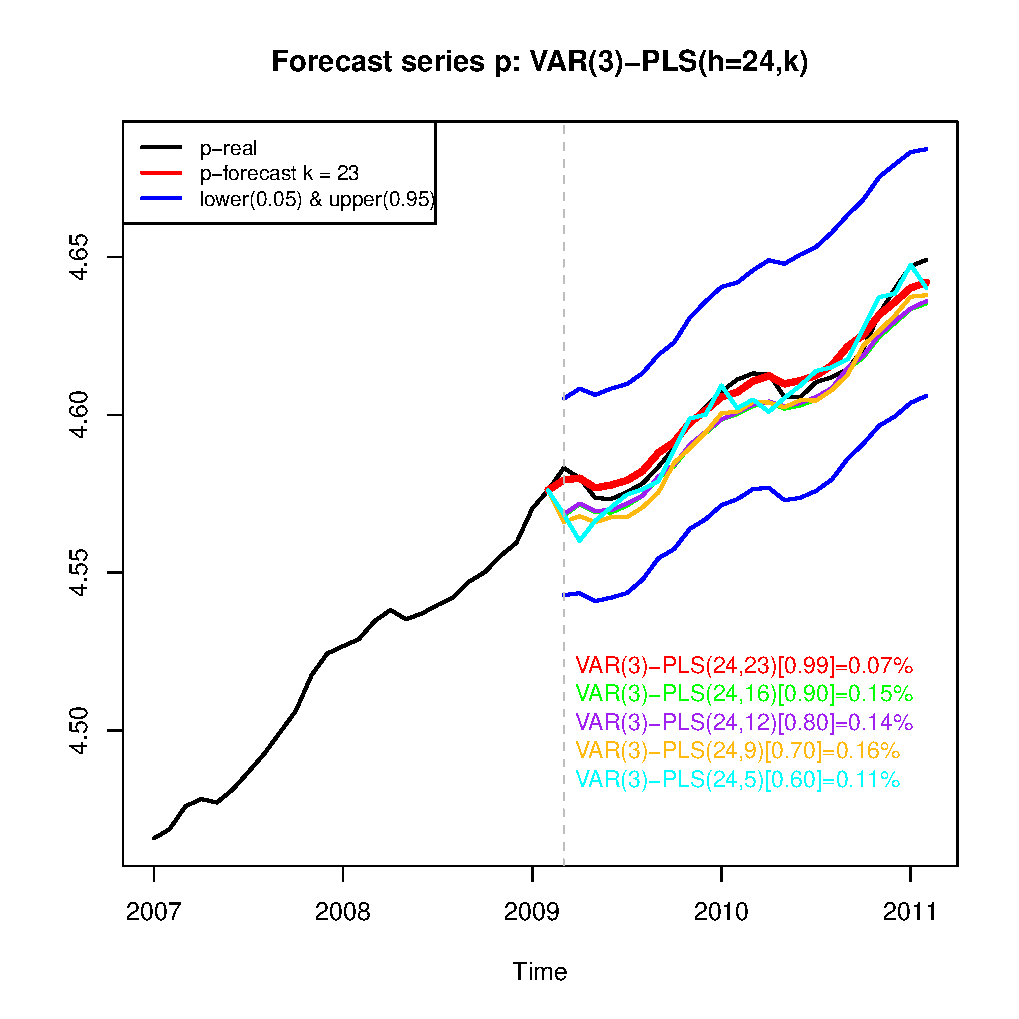
\includegraphics[scale=0.45]
      {figs/graph_2_v2.pdf}}
  \end{figure}
  \end{frame}

\begin{frame}{$VAR-PLS$ Example}
\begin{footnotesize}
    \begin{itemize}
    \item From the economic point of view, the approximation is excelent.

\item We observe that either using, $k=23$ (0.99 of the variability) 
    with an error percentage of 0.07\% or with 70\% explanation 
    with a error percentage of 0.16\%, the real value and the predicted one, 
    for practical purposes are almost identical.

\item The bootstrap interval is very well behave.
 
    \end{itemize}
  \end{footnotesize}


  \textbf{Nota: }The objective is to forecast the price, however since it is a multivariate model we also get forecast for the other 3 variables with forecast error (average of MAPE) of : 0.20\% for the monetary base, 0.60\% for industry production index and 12.03\% for the equilibrium interest rate.

\end{frame}

\begin{frame}{$VAR-PLS$ Example}
  For the Integral-VAR, the optimum $VAR_J(P)$ are
  
    \medskip

  \begin{footnotesize}
  \begin{tabular}{|l|c|c|c|c|}
    \hline
    Criterio & MAPE & MdAPE & RMSPE & RMdSPE \\
    \hline
   Statistic & 0.16 & 0.12 & 0.19 & 0.12 \\
    Variable & r & r & r & r \\
    Lags & 3 & 2 & 3 & 2 \\
    Stationality & 9 & 11 & 9 & 11 \\
    Specification & none & none & none & none \\
    \hline
  \end{tabular}
  \end{footnotesize}

  \begin{footnotesize}
  \begin{tabular}{|l|c|c|c|}
    \hline
    Criterio & MRAE & MdRAE & GMRAE \\
    \hline
    Statistic & 0.16 & 0.12 & 0.11 \\
    Variable & r & r & r \\
    Lags & 2 & 3 & 5 \\
    Stationality & 6 & 9 & 11 \\
    Specification & none& none& none \\
    \hline
  \end{tabular}
  \end{footnotesize}
  \medskip
\end{frame}

\begin{frame}{$VAR-PLS$ Example}
  \begin{figure}[htbp]
    \center{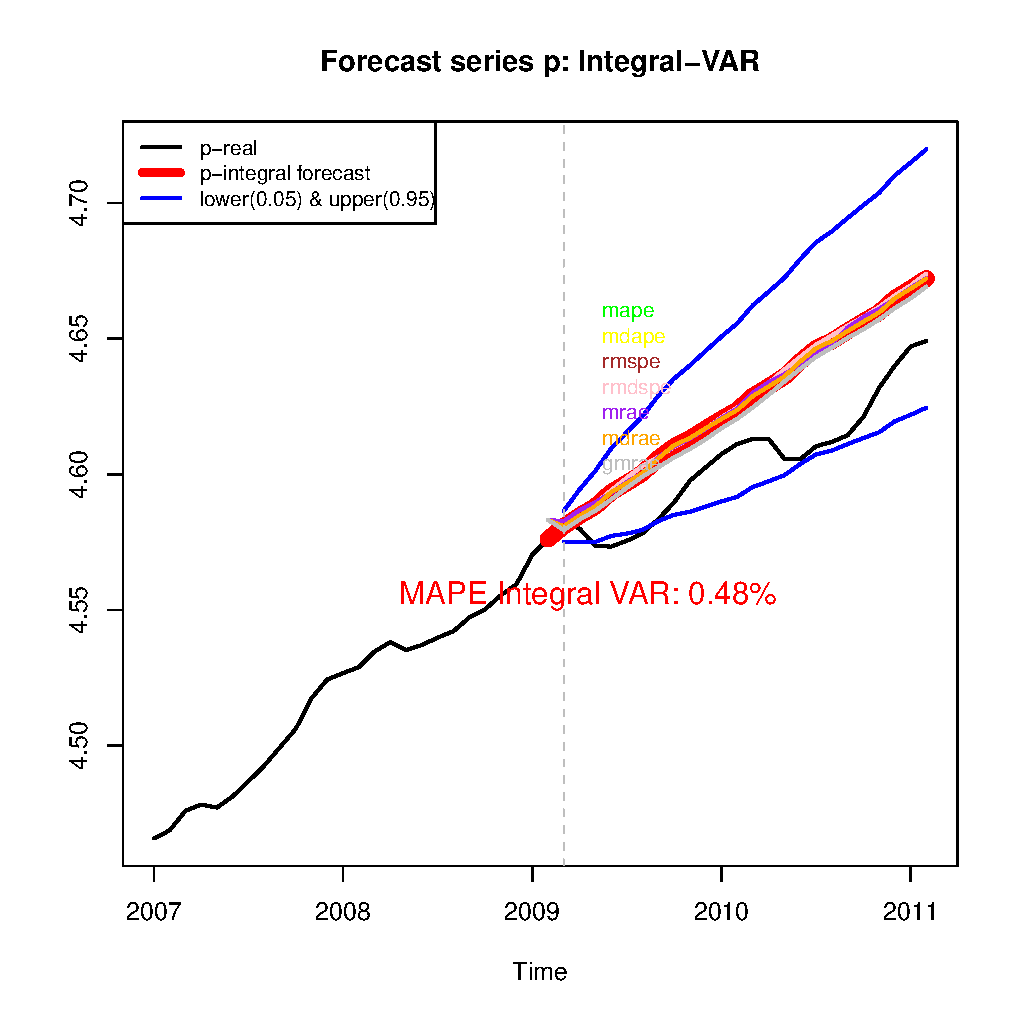
\includegraphics[scale=0.45]
      {figs/graph_3_v2.pdf}}
  \end{figure}
\end{frame}

\begin{frame}{$VAR-PLS$ Example}
  \begin{figure}[htbp]
    \center{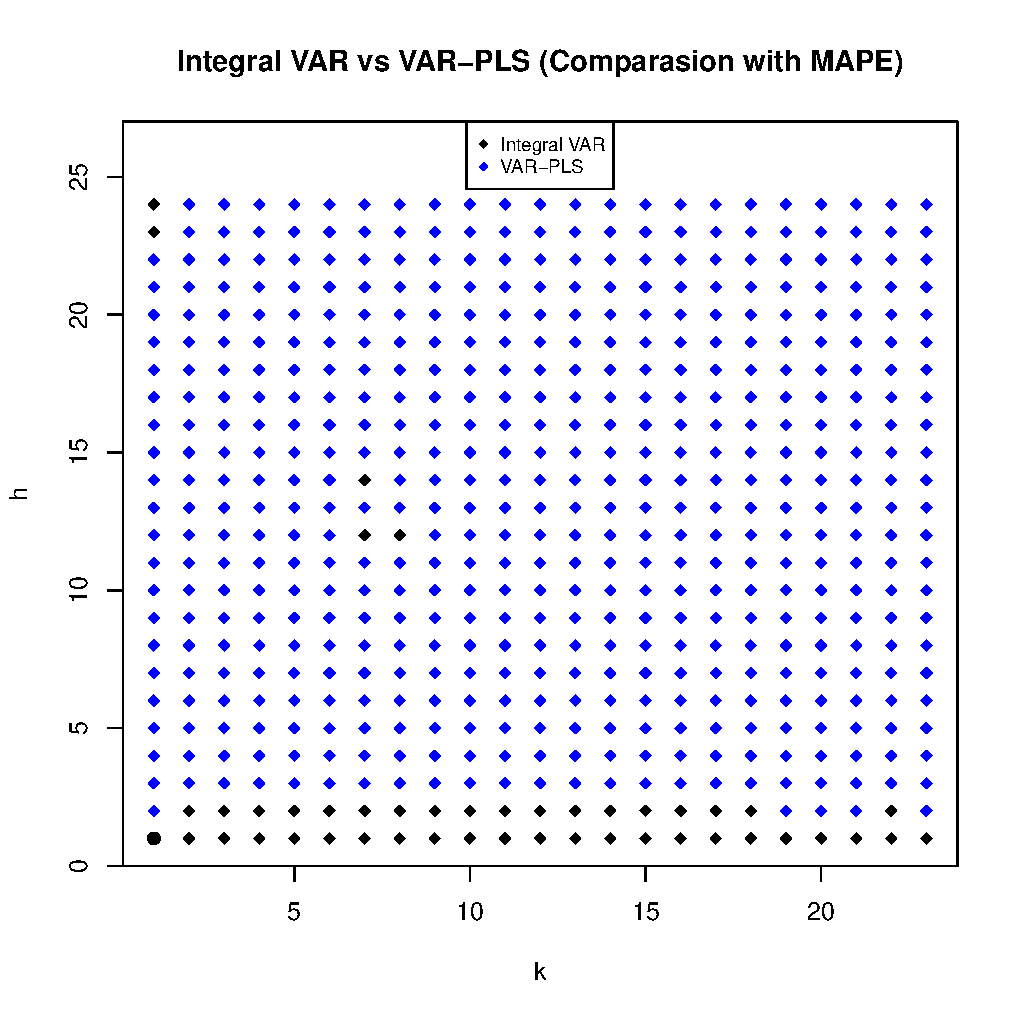
\includegraphics[scale=0.4]
      {figs/graph_4_v2.pdf}}
  \end{figure}
\end{frame}

\begin{frame}{Conclusion}
  In average 91.67\%  the PLS representation of the VAR over all the components. It make sense that the last components are less effective.

  \bigskip
  
 { \bf{CONCLUSION}}
\begin{itemize}
 \item  The  $VAR-PLS$ seems to be an attractive competitor against the integral VAR which is constructed for prediction purposes. 
  \item One the advantage is that the bootstrap prediction intervals  include the uncertainty due to the parameter estimation
  \item A second advantage is that the forecast reflect the trends and stationalites of the original series even for large number of steps ahead
  \end{itemize}
\end{frame}




\begin{frame}{}
  \begin{block}{}
    \begin{center}
      \vspace{3mm}
      {\Large Thanks !}\\
      \vspace{3mm}
    \end{center}
  \end{block}
\end{frame}




\begin{frame}{References}
\begin{footnotesize}
    \begin{itemize}
\item Bjorn Helge Mevik and Ron Wehrens The pls Package: Principal Component and Partial Least Squares Regression in R, Journal of Statistical Software January 2007, Volume 18, Issue 2. 
\item Carreiro, Kapetorios and Marcellino (2010), Forecasting Government Bond Yields with large Bayesian VAR�s. Working papers No. 662 School of Economics and Finance. 
\item Esposito Vinzi, V., W.W. Chin, J. Henseler and H. Wang (2007), Handbook of
Partial Least Squares, Berlin: Springer.
\item Philip Hans Franses (2006) Forecasting 1 to h steps ahead using partial least squares
Econometric Institute, Erasmus University Rotterdam, Econometric Institute Report 2006-47
\item P.H. Garthwaite (1994). An Interpretation of Partial Least Squares. JASA Vol 89, No 425, pp122-127 
\item Hoskuldsson (1988). PLS Regression Methods. Journal of Chemometrics, Vol 2, pp 221-228
  \end{itemize}
 \end{footnotesize}
\end{frame}

\begin{frame}{References}
\begin{footnotesize}
    \begin{itemize}

\item Kim, J.H. (2001), Bootstrap after bootstrap prediction intervals for autoregressive models, Journal of Business & Economic Statistics, 19(1), 117-128.
\item Lutkepolh, H. (1991), Introduction to Multiple Time Series Analysis, 2nd ed., Springer-
Verlag, Berlin.
\item Lutkepolh, H. (2006), Forecasting with VARMA models, in Elliot, G., C.W.J. Granger and
Timmerman (eds.), Handbook of Economic Forecasting, Vol. 1, 287-325. 
\item McIntosh A.R., Bookstein F.L., Haxby J.V.and Grady C.L. (1996). Spatial Pattern Analysis of Functional Brain Images Using Partial Least Squares NeuroImage, Volume 3, Number 3, pp. 143-157(15). Academic Press
\item Marcellino, Stock and Watson (2004), A Comparison of Direct and Iterated Multistep AR Methods for Forecasting Macroeconomic Time Series.NBER
\item Paul Nomikos and John F. MacGregor (1995) Multivariate SPC Charts for Monitoring Batch Processes Technometrics Vol. 37, No. 1, pp. 41-59

  \end{itemize}
 \end{footnotesize}
\end{frame}


\begin{frame}{References}
\begin{footnotesize}
    \begin{itemize}

\item Pascual, Ruiz y Fresoli (2011). Bootstrap forecast of multivariate VAR models without using the backward representation. Working Paper 11-34, Statistics and Econometrics Series, 
\item Pascual, L., J. Romo, and E. Ruiz (2004). Bootstrap predictive inference for ARIMA processes, Journal of Time Series Analysis, 25, 449-465
\item Pesaran, H. H., Pick, A., Timmermann, A. (2010). Variable Selection and Inference for Multi-period Forecasting Problems. Journal of Econometrics
\item Tiao, G.C., and D. Xu (1993), Robustness of maximum likelihood estimates for
multi-step predictors: the exponential case, Biometrika, 80, 623-641

   \end{itemize}
 \end{footnotesize}
 
 {\tiny Acknowledgments: Partially supported by CONACYT CB No.105657; ECO2010-19357, Spain
  and FOMIX-NL C42 -178237}
\end{frame}

\end{document}


\begin{frame}{}
  \begin{block}{}
    \begin{center}
      \vspace{3mm}
      {\Large Conclusiones}
      \vspace{3mm}
    \end{center}
  \end{block}
\end{frame}

\begin{frame}{Conclusions}
  \begin{itemize}
  \item Presentamos un algoritmo alternativo de predicci\'on para un
    entorno multivariado, que toma en cuenta las dependencias entre
    las series $y_{t+j}$ con $y_t$, mediante un modelo PLS escrito
    como un modelo lineal con $X$ teniendo la representaci\'on $VARX$.
  \item Los resultados emp\'iricos para la inflaci\'on de M\'exico son
    bastante apropiados desde un punto de vista econ\'omico.
    \begin{itemize}
    \item VAR-PLS se contruy\'o con $p$ dado por el ajuste de un VARX,
      estimando en este caso, todos los $pK$ componentes posibles.
    \item Se construy\'o el intervalo de predicci\'on usando un
      m\'etodo Bootstrap.
    \end{itemize}
  \item El modelo VAR-PLS es una t\'ecnica multivariada atractiva para
    pronosticar este tipo de datos.
  \end{itemize}
\end{frame}
